\chapter{WING DESIGN}
\label{ch2}
This report summarizes the wing design of the airplane

\section{WING LOAD DISTRIBUTION}
\label{s:ch2_wingdesign}
Schrenk method is one of the best and simple method for approximating the aerodynamic wing 
loading.
\\
According to this method, the average of the actual chord and the chord of the semi-ellipse wing 
with the same span b and area S of the wing will be taken as the chord length at any point of the 
wing.
\begin{equation} c(y) = \frac{c_{actual}(y) + c_{cell}(y)}{2} \end{equation}
and,  \[ c_{cell} = \frac{4S}{\pi b}\sqrt{1 - \left(\frac{y}{b})\right)^2} \]
where, y is the coordinate measured from wing tip, c(y) is chord length as a function of y, c is the chord length of the wing (0.14m), b is half wing span (0.58m) and S is the area of the wing (0.086$m^2$)

Since the wing is rectangular, the chord length is same throughout the wing. Hence, the eliptical approximation gives us
\begin{equation} c(y) = \frac{0.14 + c_{cell}}{2} \end{equation}
The lift per unit span of the wing is given by
\begin{equation} q = \frac{1}{2}\rho V^2C_lc(y) \end{equation}

\pagebreak
Since we are designing for maximum loads, we consider loads during take-off
\begin{itemize}
\item $\rho = 1.23$ kg/m\textsuperscript{3}
\item $V = 10.78$  m/s
\item $C_l = 2.43$
\end{itemize}
Therefore,
\begin{equation} q = 8.6\times10^{-5}(146 + \sqrt{586.5^2 - y^2}) \end{equation}
Using $\int{qdy} = L(y)$
\begin{equation}
L(y) = 8.6\times10^{-5}\left(146 + 0.315\left[\frac{y}{2}\sqrt{586.5^2 - y^2} + \frac{586.5^2}{2}sin^{-1}\frac{y}{586.5}\right]\right)
\end{equation}

where, y is in mm.

The follwing plots outline the shear force and bending moment diagrams. Fig.\ref{fig:liftdist} gives the lift distribution on the wing, Fig.\ref{fig:BMD} gives the bending moment diagram and Fig.\ref{fig:SFD} gives the shear force diagram
\begin{figure}[H]
    \begin{center}
      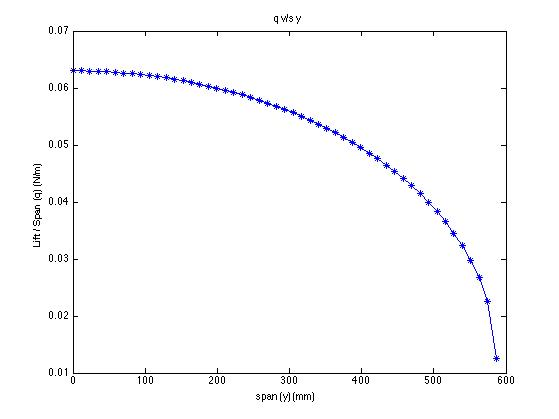
\includegraphics[width=5.1in]{figures/qy.jpg}
\caption{Lift Distribution per unit span of wing}
       \label{fig:liftdist}
    \end{center}
\end{figure}

\begin{figure}[H]
    \begin{center}
      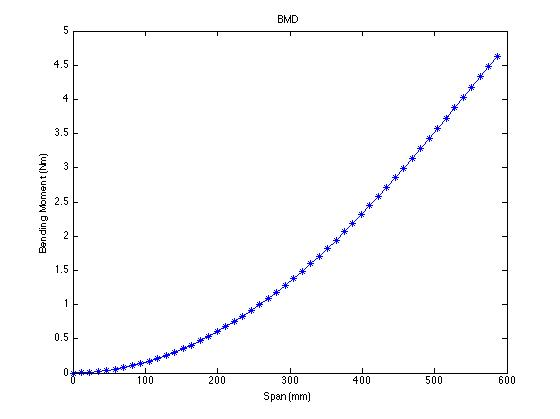
\includegraphics[width=5.1in]{figures/bmd.jpg}
\caption{Bending Moment diagram due to lift}
       \label{fig:BMD}
    \end{center}
\end{figure}
\begin{figure}[H]
    \begin{center}
      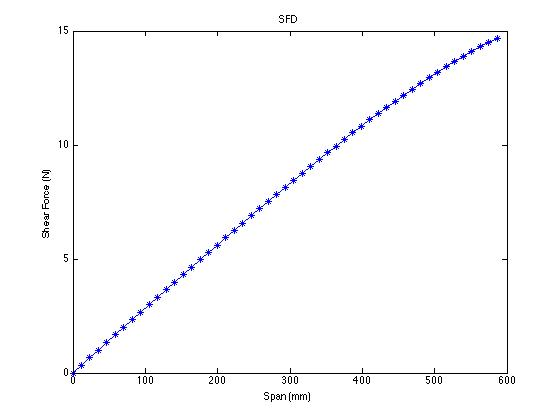
\includegraphics[width=5.1in]{figures/liftdistr.jpg}
\caption{Shear force Diagram due to lift}
       \label{fig:SFD}
    \end{center}
\end{figure}
%
\section{Spar design}
The maximum yield strength of spar material aluminium is $\sigma_{yield} = 19$ MPa. Taking a box section as the spar section, we get moment of inertia of the section as 
\begin{equation} I_{yy} = 2\left(\frac{bd^3}{12} + \frac{btd^2}{4}\right) \end{equation}
where, b is the breadth and d is the depth of the rectangular box spar. Fig.\ref{fig:spar} shows the spar cross-section.
\begin{figure}[H]
    \begin{center}
      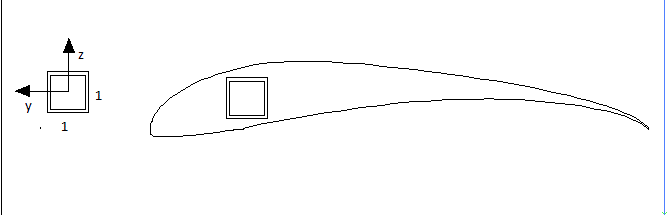
\includegraphics[width=5.2in]{figures/spar.png}
\caption{Spar cross section}
       \label{fig:spar}
    \end{center}
\end{figure}
We are using a spar section of 1cm by 1cm with a thickness of 1mm (least dimensions available on the market). Now, we need to check if this spar design is sufficient to carry all types of stresses.

\subsection{Spar under bending stress}
The maximum bending moment, $M_{max}$ is 4.62 Nm,which is calculated from the bending moment diagram. Now,
\begin{equation} \sigma = \frac{M_z}{I_{yy}}  \end{equation}
Using the spar cross section, we get
$ I_{yy} = 2.16\times10^{-9} $ m\textsuperscript{4}, $\sigma = 10.7$ MPa
.This value of bending stress is lesser than the yield stress with a factor of safety of almost 2. Hence, the spar is safe w.r.t bending stresses.

\subsection{Spar under shear stresses}
Now that we know the spar cross-section, we can plot the SFD and BMD including the weight of the aircraft. 
Using the thumb rule of 1 rib per chord of wing, we choose 8 ribs for the wing. Using balsa wood as the material, we get the ribs for the wing to weigh 1.8g. Similarly, we get the spar to be 108g. We neglect the weight of the ribs for simplicity. 
\\
The revised SFD and BMD are shown below
\begin{figure}[H]
    \begin{center}
      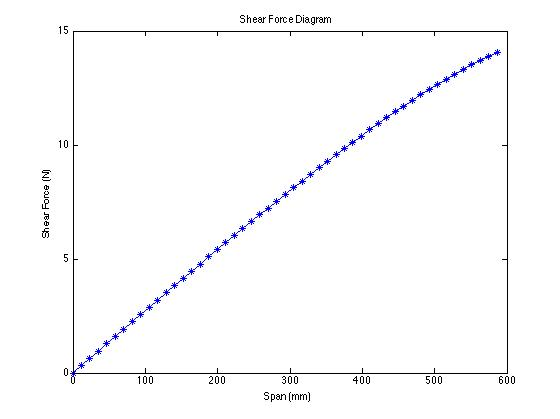
\includegraphics[width=5.1in]{figures/sfdrev.jpg}
\caption{Shear force Diagram}
       \label{fig:SFDrev}
    \end{center}
\end{figure}
\begin{figure}[H]
    \begin{center}
      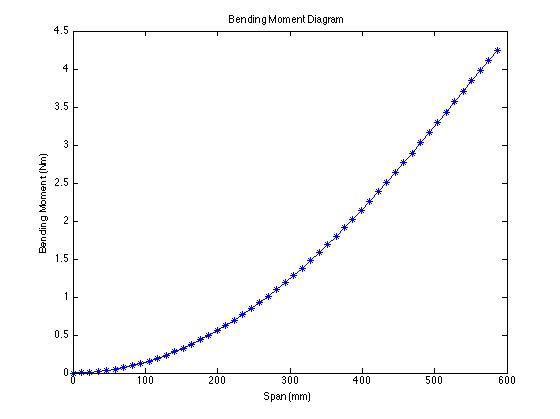
\includegraphics[width=5.1in]{figures/bmdrev.jpg}
\caption{Bending Moment diagram}
       \label{fig:BMDrev}
    \end{center}
\end{figure}

Shear stresses are caused by wing pitching moment (twist) and vertical forces. We can rule out twist due to lift forces as the spar runs through the aerodynamic center of the wing. The torque due to pitching moment is 
\begin{equation} T = \frac{1}{2}\rho v^2SC_mc \end{equation}
The shear flow through the section is given by
\begin{equation} q = -\frac{V_zt}{I_{yy}}\int{yds} + \frac{T}{2A} \end{equation}
where, $V_z = 14.06$ N, $t = 1$ mm, $T = 0.48$ Nm, $A = 1$ cm\textsuperscript{2}\\
\begin{figure}[H]
    \begin{center}
      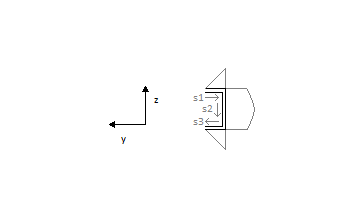
\includegraphics[width=5.2in]{figures/airfoil_stress.png}
\caption{Shear flow around spar section}
       \label{fig:shearflow}
    \end{center}
\end{figure}
A standard shear flow analysis gives us
\[ q_1 = -32.4s_1\]
\[ q_2 = -6.48(5s_2 - 0.5s_2^2)-162\]
where, s is in mm and as directed in \ref{fig:shearflow}. The maximum shear stress is calculated from the shear flow using
\begin{equation} \tau_{max} = q_{max}/t \end{equation}
Looking at the shear flow, we get $q_{max} = 243$ N/m (at $s_2 = 5$ mm) and due to torque $q = 2398$ N/m, Hence, $q_{total} = 2641$ N/m and therfore $\tau_{max} = 2.641$ MPa

\subsection{Spar under buckling stresses - web}
To check if the spar web buckles, we use the following web buckling formula
\begin{equation} \sigma_{max} = KE\left(\frac{t}{b}\right)^2 \end{equation}
Substituting, K = 3.67 and E = 70 GPa for Aluminium, we get $\sigma_{max} = 2.6$ GPa \\

The maximum stresses are far lesser than this. Thus, we conclude that no buckling problems will be encountered for the spar.
%
%
